\documentclass[11pt,letterpaper]{article}

\usepackage[margin=1in,headheight=14pt]{geometry}
\usepackage{amsmath,amssymb,amsthm,mathtools}
\usepackage{graphicx}
\usepackage{xcolor}
\usepackage{enumitem}
\usepackage{microtype}
\usepackage{fancyhdr}
\usepackage[colorlinks=true,linkcolor=blue,citecolor=blue,urlcolor=blue]{hyperref}

% Personal notation and theorem environments.
%!TEX root = EM_singular_models.tex

% PDF margin etc settings
%\setlength{\textwidth}{\paperwidth}
%\addtolength{\textwidth}{-6cm}
%\setlength{\textheight}{\paperheight}
%\addtolength{\textheight}{-4cm}
%\addtolength{\textheight}{-1.1\headheight}
%\addtolength{\textheight}{-\headsep}
%\addtolength{\textheight}{-\footskip}
%\setlength{\oddsidemargin}{0.5cm}
%\setlength{\evensidemargin}{0.5cm}

%%%%%%%%%%%%%%%%%%%%%%%%%%%%%%%%

% MACROS HERE

%%%%%%%%%%%%%%%%%%%%%%%%%%%%%%%%

\newcommand{\fixedpointtheta}{\widehat\theta_\obs}

\newcommand{\cover}{N}
\newcommand{\kinit}{\nu}
\newcommand{\cdelta}{c_\threshold}
\newcommand{\dndelta}{\omega}
\newcommand{\kndelta}{\Upsilon}
\newcommand{\kndeltanew}{\Psi}
\newcommand{\radii}{\mathcal{R}}
\newcommand{\event}{\mathcal{E}}
\newcommand{\kevent}{\mathcal{D}}


% Observations, dimension etc.
\newcommand{\dims}{\ensuremath{d}}
\newcommand{\samples}{\ensuremath{n}}
\newcommand{\obs}{\samples}
\newcommand{\real}{\ensuremath{\mathbb{R}}}
\newcommand{\complex}{\ensuremath{\mathbb{C}}}
\newcommand{\realdim}{\ensuremath{\real^\dims}}

\newcommand{\smallthreshold}{\epsilon}

% some mathcal notations
\newcommand{\order}[1]{\ensuremath{\mathcal{O}\parenth{#1}}}

% Basic statistics notation
\newcommand{\xstar}{\ensuremath{x^*}}
\newcommand{\xbar}{\ensuremath{\bar{x}}}
% True parameter
\newcommand{\thetastar}{\ensuremath{{\theta^*}}}
% Estimate one
\newcommand{\thetahat}{\ensuremath{\widehat{\theta}}}
% Estimate two
\newcommand{\thetatil}{\ensuremath{\widetilde{\theta}}}
\newcommand{\thetabar}{\ensuremath{\bar{\theta}}}
\newcommand{\yvec}{\ensuremath{y}}
\newcommand{\Xmat}{\ensuremath{X}}

% Distributions
\newcommand{\distribution}{P}
\newcommand{\density}{f}
\newcommand{\gaussiandensity}{\phi}
\newcommand{\NORMAL}{\ensuremath{\mathcal{N}}}
\newcommand{\BER}{\ensuremath{\mbox{Ber}}}

% Spaces
\newcommand{\Xspace}{\ensuremath{\mathcal{X}}}
\newcommand{\Yspace}{\ensuremath{\mathcal{Y}}}
\newcommand{\Zspace}{\ensuremath{\mathcal{Z}}}


% Brackets Size
\newcommand{\brackets}[1]{\left[ #1 \right]}
\newcommand{\parenth}[1]{\left( #1 \right)}
\newcommand{\bigparenth}[1]{\big( #1 \big)}
\newcommand{\biggparenth}[1]{\bigg( #1 \bigg)}
\newcommand{\braces}[1]{\left\{ #1 \right \}}
\newcommand{\abss}[1]{\left| #1 \right |}
\newcommand{\angles}[1]{\left\langle #1 \right \rangle}
\newcommand{\tp}{^\top}

% Generic vectors and scalars
\newcommand{\myvec}{u} % for generic vector
\newcommand{\myvectwo}{v} % for generic vector
\newcommand{\mymat}{B}
\newcommand{\set}{{A}}
\newcommand{\scalar}{\alpha}
\newcommand{\tvscalar}{\epsilon}
\newcommand{\tailboundscalar}{t}
\newcommand{\term}{U}
\newcommand{\myVarone}{\alpha_X}
\newcommand{\myVartwo}{\alpha_Y}
\newcommand{\myCovmat}{\Sigma}
\newcommand{\xcord}[1]{x^{(#1)}}
\newcommand{\xcordpop}[1]{X^{(#1)}}
\newcommand{\ycordpop}[1]{Y^{(#1)}}
\newcommand{\myVarthree}{\ensuremath{U}}
\newcommand{\myVarfour}{\ensuremath{V}}
\newcommand{\myfuntwo}{\ensuremath{g}}
\newcommand{\numsteps}{t}
\newcommand{\totalnumsteps}{T}
\newcommand{\seqalpha}[1]{\alpha_{#1}}
\newcommand{\seqnu}[1]{\nu^{(#1)}}
\newcommand{\imax}{\ell_\smallthreshold}
\newcommand{\basis}{e}
\newcommand{\radem}{\varepsilon}
\newcommand{\Tone}{T\ensuremath{_{0}}}
\newcommand{\Ttwo}{T\ensuremath{_{2}}}
\newcommand{\contractPar}[1]{\ensuremath{\gamma\parenth{#1}}}

\newcommand{\simiid}{\overset{\mathrm{i.i.d.}}{\sim}}
\newcommand{\eqd}{\overset{d}{=}}


% EM updates
\newcommand{\hidden}{Z}
\newcommand{\qfun}[2]{Q(#1\vert#2)}
\newcommand{\variable}{\theta}
\newcommand{\weights}{w}
\newcommand{\myfun}{q}
\newcommand{\gradf}{\nabla \myfun}
\newcommand{\hessf}{\nabla^2 \myfun}
\newcommand{\iter}{t}
\newcommand{\mupdate}{M}
\newcommand{\mupdategeneral}{\ensuremath{M^{GN}}}




% EM contractions
\newcommand{\contractgene}{\ensuremath{\gamma^{GN}}}
\newcommand{\updateMat}{\ensuremath{\Gamma_{\theta}}}
\newcommand{\mymatTheta}{\ensuremath{B_{\theta}}}
\newcommand{\sech}{\text{sech}}

% Nhat's macros 
\newcommand{\Rspace}{\ensuremath{\mathbb{R}}}
\newcommand{\Ecal}{\ensuremath{\mathcal{E}}}
\newcommand{\Ncal}{\ensuremath{\mathcal{N}}}
\newcommand{\gradient}{\ensuremath{\nabla}}
\newcommand{\smallweight}{\ensuremath{\epsilon^{sw}}}
\newcommand{\smallnorm}{\ensuremath{\rho^{sw}}}
\newcommand{\ball}{\ensuremath{\mathbb{B}}}
\newcommand{\sphere}{\ensuremath{\mathbb{S}}}

\newcommand{\diam}{\ensuremath{\text{diam}}}
\newcommand{\upper}{\ensuremath{\bar{C}}}
\newcommand{\sample}{\ensuremath{\xi}}
\newcommand{\weight}{\ensuremath{\pi}}
\newcommand{\contracasym}{\ensuremath{\rho}}
\newcommand{\Fishermatrix}{\ensuremath{\mathcal{I}}}
\newcommand{\barcontracasym}{\ensuremath{\bar{\rho}}}


\newcommand{\TrueDensity}{\ensuremath{f}}
\newcommand{\FitDensity}{\ensuremath{f}_{\theta}}
\newcommand{\FitDensityfree}{\ensuremath{f}_{\pi, \theta}}
\newcommand{\FitDensitygen}{\ensuremath{f}_{\pi, \theta_{1}, \theta_{2}}}
\newcommand{\FitDensitymore}{\ensuremath{f}_{G}}
\newcommand{\normden}{\ensuremath{\phi}}
\newcommand{\mean}{\ensuremath{\theta}}
\newcommand{\sd}{\ensuremath{\sigma}}
\newcommand{\parFOS}{\ensuremath{\gamma}}
\newcommand{\funQ}{\ensuremath{Q}}
\newcommand{\updateM}{\ensuremath{M}}
\newcommand{\weightFun}{\ensuremath{w}}
\newcommand{\mydefn}{\ensuremath{:=}}
\newcommand{\poincare}{\ensuremath{\tilde{C}}}
\newcommand{\paraspace}{\ensuremath{\Theta}}
\newcommand{\loglihood}{\ensuremath{F}}
\newcommand{\prior}{\ensuremath{\pi}}
\newcommand{\posterior}{\ensuremath{\Pi}}
\newcommand{\boundcons}{\ensuremath{B}}
\newcommand{\boundconstot}{\ensuremath{H}}
\newcommand{\noise}{\ensuremath{\varepsilon}}
\newcommand{\loglihoodgaus}{\ensuremath{F^{G}}}
\newcommand{\loglihoodind}{\ensuremath{F^{I}}}
\newcommand{\loglihoodlogit}{\ensuremath{F^{R}}}
\newcommand{\noiseone}{\ensuremath{\varepsilon_{1}}}
\newcommand{\noisetwo}{\ensuremath{\varepsilon_{2}}}

%%%SDE_Bayesian_inf
\newcommand{\weakcon}{\ensuremath{\psi}}
\newcommand{\perturb}{\ensuremath{\zeta}}
\newcommand{\inver}{\ensuremath{\xi}}

% Universal constants
\newcommand{\unicon}{c}
\newcommand{\uniconnew}{c'}
\newcommand{\uniconone}{c_1}
\newcommand{\unicontwo}{c_2}

% some parameters that you may define
\newcommand{\scparam}{m} % strong  convexity parameter
\newcommand{\smoothness}{L} % smoothness parameter
\newcommand{\step}{h}


%%%%%%%%% Distributions and Random variables %%%%%%%%%%%
\newcommand{\rvg}{\xi} % to denote the random variable g
\newcommand{\threshold}{\delta}


%%%%%%%%% Basic Terms like defn, etal, tmix, polylog %%%%%%%%%%%
\newcommand{\defn}{:=}
\newcommand{\rdefn}{=:}
\newcommand{\etal}{{et al.}}
\newcommand{\polylog}{\text{poly-log}}

% Some vector/matrix norms
\newcommand{\matnorm}[3]{|\!|\!| #1 | \! | \!|_{{#2}, {#3}}}
\newcommand{\matsnorm}[2]{|\!|\!| #1 | \! | \!|_{{#2}}}
\newcommand{\vecnorm}[2]{\left\| #1\right\|_{#2}}
\newcommand{\enorm}[1]{\vecnorm{#1}{2}} % euclidean norm
\newcommand{\nucnorm}[1]{\ensuremath{\matsnorm{#1}{\footnotesize{\mbox{nuc}}}}}
\newcommand{\fronorm}[1]{\ensuremath{\matsnorm{#1}{\footnotesize{\mbox{fro}}}}}
\newcommand{\opnorm}[1]{\ensuremath{\matsnorm{#1}{\tiny{\mbox{op}}}}}
%%% EM paper
\newcommand{\constrainnorm}[1]{\vecnorm{#1}{[k]}} % euclidean norm

\newcommand{\bigmatsnorm}[2]{{\Big|\!\Big|\!\Big| #1
  \Big|\!\Big|\!\Big|}_{#2}}

% Inner product
\newcommand{\inprod}[2]{\ensuremath{\langle #1 , \, #2 \rangle}}

% Kullback-Leibler
\newcommand{\kull}[2]{\ensuremath{D_{\text{KL}}(#1\; \| \; #2)}}

% Probability
\newcommand{\Exs}{\ensuremath{{\mathbb{E}}}}
\newcommand{\Prob}{\ensuremath{{\mathbb{P}}}}

%Eigenvector / eigenvalue related notation
\newcommand{\eig}[1]{\ensuremath{\lambda_{#1}}}
\newcommand{\eigmax}{\ensuremath{\eig{\max}}}
\newcommand{\eigmin}{\ensuremath{\eig{\min}}}

% \DeclareMathOperator{\det}{det}
\DeclareMathOperator{\modd}{mod}
\DeclareMathOperator{\diag}{diag}
\DeclareMathOperator{\var}{var}
\DeclareMathOperator{\cov}{cov}
\DeclareMathOperator{\trace}{trace}
\DeclareMathOperator{\abs}{abs}
\DeclareMathOperator{\floor}{floor}
\DeclareMathOperator{\vol}{vol}
\DeclareMathOperator{\child}{child}
\DeclareMathOperator{\parent}{parent}
\DeclareMathOperator{\sign}{sign}
\DeclareMathOperator{\rank}{rank}
\DeclareMathOperator{\toeplitz}{toeplitz}




\newtheoremstyle{named}{}{}{\itshape}{}{\bfseries}{.}{.5em}{\thmnote{#3's }#1}
\theoremstyle{named}
\newtheorem*{namedtheorem}{Lemma}

%%%%%%%
\theoremstyle{plain}

% {Theorem, Proposition, Lemma, Corollary} numbered sequentially
% throughout the paper
\newtheorem{theorem}{Theorem}
\newtheorem{proposition}{Proposition}
\newtheorem{lemma}{Lemma}
\newtheorem{claim}{Claim}
\newtheorem{corollary}{Corollary}
\newtheorem{definition}{Definition}
\newtheorem{conjecture}{Conjecture}
\newtheorem{remark}{Remark}
%%%%%%%%%%%%%%%%%%%%%%%%%%%%%%%%%%%%%%%%%%%%%%%%%%%%%%%%%%%%%%%%%%%%%%%
% WIDEBAR COMMAND
\newlength{\widebarargwidth}
\newlength{\widebarargheight}
\newlength{\widebarargdepth}
\DeclareRobustCommand{\widebar}[1]{%
  \settowidth{\widebarargwidth}{\ensuremath{#1}}%
  \settoheight{\widebarargheight}{\ensuremath{#1}}%
  \settodepth{\widebarargdepth}{\ensuremath{#1}}%
  \addtolength{\widebarargwidth}{-0.3\widebarargheight}%
  \addtolength{\widebarargwidth}{-0.3\widebarargdepth}%
  \makebox[0pt][l]{\hspace{0.3\widebarargheight}%
    \hspace{0.3\widebarargdepth}%
    \addtolength{\widebarargheight}{0.3ex}%
    \rule[\widebarargheight]{0.95\widebarargwidth}{0.1ex}}%
  {#1}}



%%% New version of \caption puts things in smaller type, single-spaced
%%% and indents them to set them off more from the text.
\makeatletter
\long\def\@makecaption#1#2{
        \vskip 0.8ex
        \setbox\@tempboxa\hbox{\small {\bf #1:} #2}
        \parindent 1.5em  %% How can we use the global value of this???
        \dimen0=\hsize
        \advance\dimen0 by -3em
        \ifdim \wd\@tempboxa >\dimen0
                \hbox to \hsize{
                        \parindent 0em
                        \hfil
                        \parbox{\dimen0}{\def\baselinestretch{0.96}\small
                                {\bf #1.} #2
                                %%\unhbox\@tempboxa
                                }
                        \hfil}
        \else \hbox to \hsize{\hfil \box\@tempboxa \hfil}
        \fi
        }
\makeatother



%% COMMENTING commands

\long\def\comment#1{}
\definecolor{battleshipgrey}{rgb}{0.52, 0.52, 0.51}
\definecolor{darkgray}{rgb}{0.66, 0.66, 0.66}
\definecolor{darkgreen}{rgb}{0.0, 0.2, 0.13}
\definecolor{darkspringgreen}{rgb}{0.09, 0.45, 0.27}
\definecolor{dukeblue}{rgb}{0.0, 0.0, 0.61}
\definecolor{olivedrab7}{rgb}{0.24, 0.2, 0.12}
\definecolor{darkblue}{rgb}{0.0, 0.0, 0.55}
\definecolor{darkscarlet}{rgb}{0.34, 0.01, 0.1}
\definecolor{candyapplered}{rgb}{1.0, 0.03, 0.0}
\definecolor{ao(english)}{rgb}{0.0, 0.5, 0.0}
\definecolor{applegreen}{rgb}{0.55, 0.71, 0.0}

\newcommand{\red}[1]{\textcolor{red}{#1}}
\newcommand{\mjwcomment}[1]{{\bf{{\red{{MJW --- #1}}}}}}
\newcommand{\mwlcomment}[1]{{\bf{{\color{orange}{{Wenlong --- #1}}}}}}

\newcommand{\blue}[1]{\textcolor{blue}{#1}}
\newcommand{\green}[1]{\textcolor{green}{#1}}
\newcommand{\highlight}[1]{\textcolor{applegreen}{#1}}

% comment lines
\newcommand{\genecomment}[1]{{\bf{{\blue{{TEAM --- #1}}}}}}
\newcommand{\rrdcomment}[1]{{\bf{{\blue{{RRD --- #1}}}}}}
\newcommand{\nhcomment}[1]{{\bf{{\blue{{NH --- #1}}}}}}
\newcommand{\kkcomment}[1]{{\bf{{\darkgreen{{KK --- #1}}}}}}


\newcommand{\widgraph}[2]{\includegraphics[keepaspectratio,width=#1]{#2}}


\newcommand{\coursenumber}{STA3000F}
\newcommand{\coursetitle}{Advanced Theory of Statistics}
\newcommand{\courseterm}{Fall 2026}
\newcommand{\lecturenumber}{2}
\newcommand{\lecturedate}{September 18, 2026}
\newcommand{\lecturer}{Wenlong Mou}

\pagestyle{fancy}
\fancyhf{}
\fancyhead[L]{\coursenumber: \coursetitle}
\fancyhead[R]{Lecture \lecturenumber}
\fancyfoot[C]{\lecturenumber--\arabic{page}}
\renewcommand{\headrulewidth}{0.4pt}
\renewcommand{\footrulewidth}{0pt}

\usepackage{bm}

\setcounter{section}{0}
\renewcommand{\thepage}{\lecturenumber--\arabic{page}}

\newtheorem{example}{Example}

\newcommand{\makelecturenotesheader}{%
  \noindent
  \textbf{\coursenumber: \coursetitle}%
  \hfill
  \textbf{\courseterm}

  \begin{center}
    {\Large\bfseries Lecture \lecturenumber: \lecturedate}
  \end{center}

  \noindent
  \textbf{Lecturer:} \lecturer
  \par\medskip
  \hrule
  \bigskip
}

\begin{document}

\makelecturenotesheader

\section{Decision theory continued}
Continued from last time.
\begin{example}
  Consider $X_1, X_2, \cdots, X_n \simiid \mathcal{N} (\theta, 1)$ with unknown $\theta \in \real$. Prior distribution $\pi = \mathcal{N} (0, \tau^2)$. Posterior becomes
  \begin{align*}
    \Pi (\theta \mid X_1^n) \propto \pi (\theta) \cdot p_\theta (X_1) p_\theta (X_2) \cdots p_\theta (X_n) = \mathcal{N} \Big( \frac{\tau^2 n \bar{X}_n}{\tau^2n + 1}, \frac{\tau^2}{\tau^2 n + 1} \Big).
  \end{align*}
  Posterior mean (Bayes optimal w.r.t. $\pi$) is
  \begin{align*}
    \thetahat_\pi = \frac{\tau^2 n \bar{X}_n}{\tau^2 n + 1} = \Big( 1 - \frac{1}{\tau^2 n + 1} \Big) \bar{X}_n.
  \end{align*}
  This is also a shrinkage estimator, with fixed shrinkage factor $1/(\tau^2 n + 1)$. c.f. James--Stein estimator, which has a data-dependent shrinkage factor.
\end{example}
Remarks: In general, you can use conjugate prior-likelihood pairs to get closed-form posterior distribution. For example, for Bernoulli likelihood, use Beta prior; for Poisson likelihood, use Gamma prior; for Gaussian likelihood with unknown mean and variance, use Normal-Inverse-Gamma prior.

\subsection{Minimax decision rules}
Idea: instead of minimizing the Bayes risk, we can minimize the worst-case risk.
\begin{align*}
    r_{\mathrm{minimax}} \mydefn \inf_\delta~ \sup_{\theta \in \Theta} R(\theta; \delta).
\end{align*}
Note that the order of $\inf$ and $\sup$ cannot be exchanged in general. Game-theoretic interpretation:
\begin{itemize}
  \item Statistician first chooses a decision rule $\delta$ without knowing the nature's choice.
  \item Nature (after observing $\delta$) chooses a parameter $\theta \in \Theta$ to maximize the risk.
\end{itemize}
In general, you can also consider randomized strategy for the nature (and statistician). (e.g. in rock-paper-scissors game, the optimal strategy is to randomize uniformly over the three choices.)
\begin{align*}
    r_{\mathrm{minimax}} = \inf_\delta~ \sup_{\theta \in \Theta} R(\theta; \delta) = \inf_\delta~ \sup_{\pi} \int_\Theta R(\theta; \delta) d\pi(\theta) = \inf_\delta~ \sup_{\pi} r_\pi (\delta).
\end{align*}
Weak duality:
\begin{align*}
    \inf_\delta~ \sup_{\pi} r_\pi (\delta) \geq \sup_{\pi}~ \inf_\delta r_\pi (\delta).
\end{align*}
In game theory, there's well-known result that gives us strong duality.
\begin{theorem}[von Neumann's minimax theorem, simplified version]
  If $\Theta, \mathbb{X}, \mathbb{A}$ are all finite. Then we have
  \begin{align*}
    \inf_\delta~ \sup_{\pi} r_\pi (\delta) = \sup_{\pi}~ \inf_\delta r_\pi (\delta).
  \end{align*}
\end{theorem}
This can be extended to continuous cases assuming certain compactness, convexity, and regularity assumptions.

What does it tell us in terms of statistics? Minimax risk is the worst-case Bayes risk.

\subsection{Some sufficient conditions for minimax rules}
\begin{proposition}
  A constant-risk Bayes rule is minimax.
\end{proposition}
Proof: Consider another decision rule $\delta'$. Then, we have
\begin{align*}
    \sup_{\theta \in \Theta} R(\theta; \delta') \geq \int_\Theta R(\theta; \delta') d\pi(\theta) \geq r_\pi (\delta_\pi) = \sup_{\theta \in \Theta} R(\theta; \delta_\pi).
\end{align*}
This shows that the Bayes rule $\delta_\pi$ is minimax.
\begin{example}\upshape
  Consider $X \sim \mathrm{Binom} (n, p)$ with known $n$ and unknown $p \in [0, 1]$. The goal is to estimate $p$ under squared error loss.

  Natural choice of estimator is $\widehat{p} = X/n$. The risk function is
  \begin{align*}
    R(p; \widehat{p}) = \Exs_{X \sim \mathrm{Binom}(n, p)} \Big[ \Big( \frac{X}{n} - p \Big)^2 \Big] = \frac{p(1 - p)}{n}.
  \end{align*}
  This is not a constant-risk estimator.

  To find minimax estimator, we can consider a prior distribution $\pi = \mathrm{Beta}(\alpha, \beta)$. Then, the Bayes estimator is
  \begin{align*}
    \widehat{p}_\pi = \frac{X + \alpha}{n + \alpha + \beta}.
  \end{align*}
\end{example}
The risk function of $\widehat{p}_\pi$ is
\begin{align*}
  R(p; \widehat{p}_\pi) = \Exs_{X \sim \mathrm{Binom}(n, p)} \Big[ \Big( \frac{X + \alpha}{n + \alpha + \beta} - p \Big)^2 \Big] = \frac{np(1 - p) + (\alpha - (\alpha + \beta)p)^2}{(n + \alpha + \beta)^2}.
\end{align*}
By choosing $\alpha = \beta = \sqrt{n}/2$, we have
\begin{align*}
  R(p; \widehat{p}_\pi)  = \frac{1}{4(1 + \sqrt{n})^2} = r_{\mathrm{minimax}}.
\end{align*}
\begin{center}
  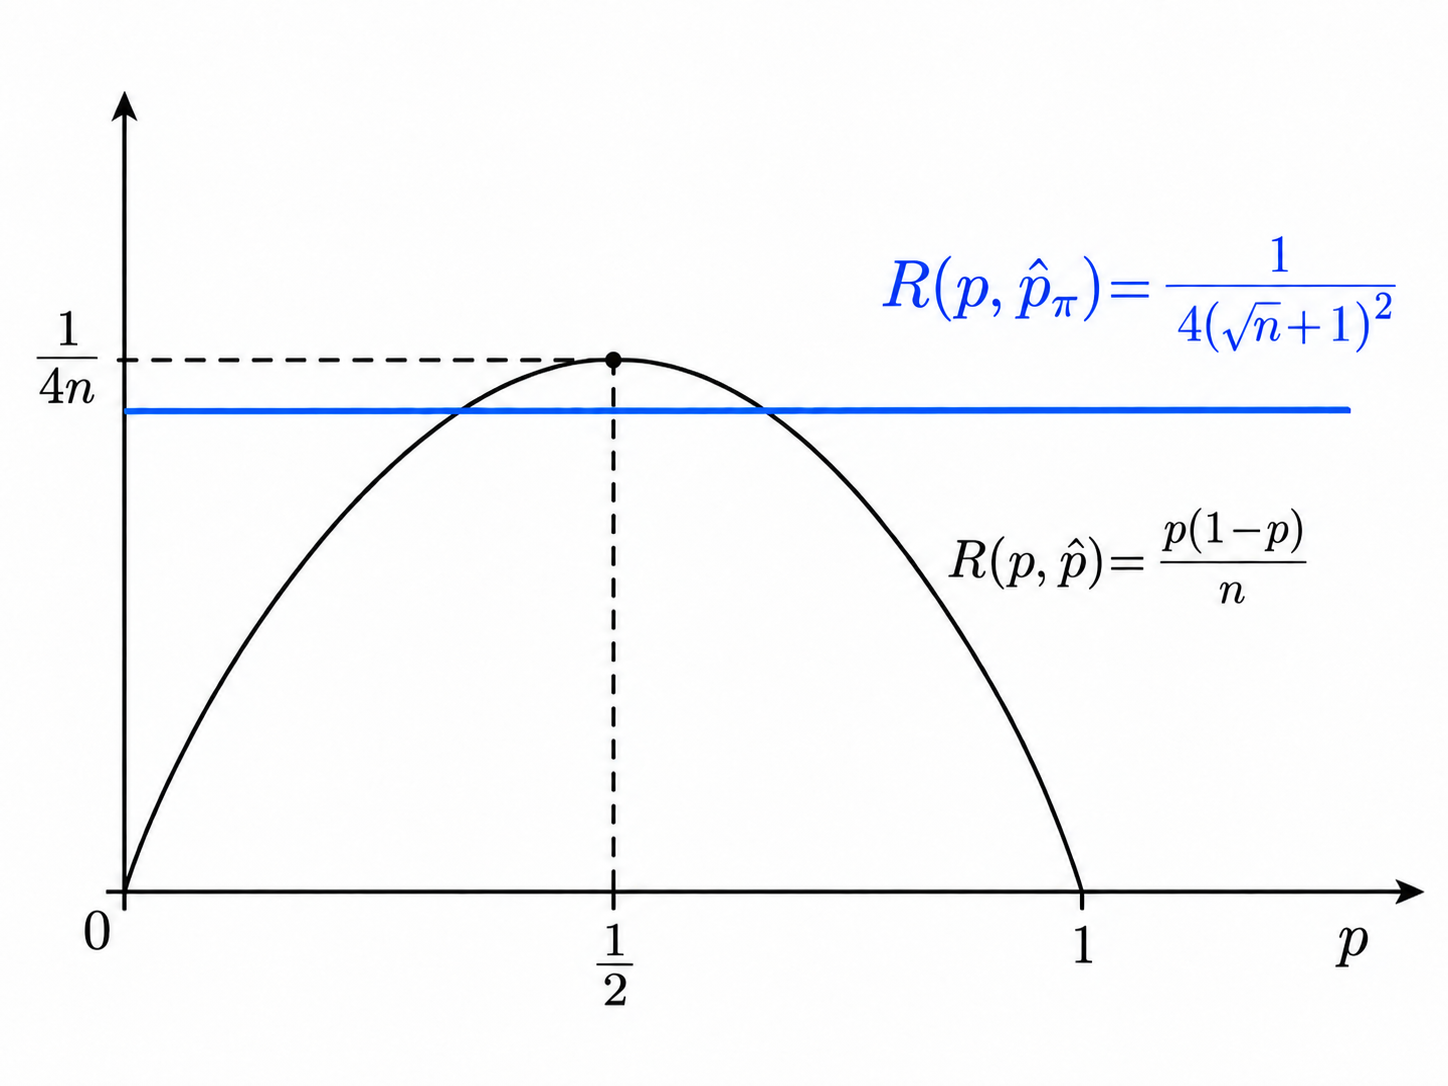
\includegraphics[width=0.78\textwidth]{./lec2-binomial-minimax-illustration.png}

  \small Risk comparison for estimating a binomial proportion: the Bayes estimator with $\alpha = \beta = \sqrt{n}/2$ has constant risk below the worst-case risk of the sample proportion.
\end{center}

Remark: does it mean that we should always use the Bayes estimator with $\mathrm{Beta}(\sqrt{n}/2, \sqrt{n}/2)$ prior? Not necessarily.

This is the problem of forcing estimators to be exact minimax, instead of the problem of sample frequency estimator.

To solve this problem, we also use approximate versions of minimax (e.g. minimax up to constant factors), and local minimax estimators (i.e., minimax estimators in a local neighborhood of the parameter space).

\begin{proposition}
  Suppose that there exist a sequence of priors $(\pi_n)_{n \geq 1}$ such that the corresponding Bayes risk $\big(r_{\pi_n} \big)_{n \geq 1}$. Suppose that there exists a decision rule $\delta$ such that
  \begin{align*}
    \lim\inf_{n \rightarrow \infty} r_{\pi_n} \geq \sup_{\theta \in \Theta} R(\theta; \delta).
  \end{align*}
  Then $\delta$ is minimax.
\end{proposition}
Proof: For any decision rule $\delta'$, we have
\begin{align*}
  \sup_{\theta \in \Theta} R(\theta; \delta') \geq \lim\inf_{n \rightarrow \infty} \int_\Theta R (\theta, \delta') d\pi_n (\theta) \geq \lim\inf_{n \rightarrow \infty} r_{\pi_n} \geq \sup_{\theta \in \Theta} R(\theta; \delta).
\end{align*}
So $\delta'$ has larger worst-case risk than $\delta$. This shows that $\delta$ is minimax.

\begin{example}
  Let $X_1, X_2, \cdots, X_n \simiid \mathcal{N} (\theta, I_d)$ with unknown $\theta \in \real^d$. We let $\pi_k = \mathcal{N} (0, k I_d)$. We can compute the Bayes risk
  \begin{align*}
  r_{\pi_k} = \frac{k d}{k n + 1} \xrightarrow{k \rightarrow + \infty} \frac{d}{n}.
  \end{align*}
On the other hand, the sample mean estimator $\widebar{X}_n$ has risk function
\begin{align*}
  R(\theta; \widebar{X}_n) = \Exs_{X \sim P_\theta} [\vecnorm{\widebar{X}_n - \theta}{2}^2] = \frac{d}{n}.
\end{align*}
So by the proposition above, $\widebar{X}_n$ is minimax.
\end{example}
Remark: a minimax estimator is no necessarily admissible (c.f. Stein's paradox).

\subsection{Relation between different criteria}
\begin{proposition}
  If $\delta$ is a unique Bayes rule with respect to a prior $\pi$. Then $\delta$ is admissible.
\end{proposition}
Proof: suppose that there exists another decision rule $\delta'$ that dominates $\delta$. Then, we have
\begin{align*}
 r_\pi (\delta') = \int_\Theta R(\theta; \delta') d\pi(\theta) \leq \int_\Theta R(\theta; \delta) d\pi(\theta) = r_\pi (\delta),
\end{align*}
By uniqueness, we have $\delta' = \delta$.
\begin{proposition}
  When $\Theta$ is finite, any admissible decision rule is a Bayes rule with respect to some prior $\pi$.
\end{proposition}
Proof: Consider the set of all risk functions
\begin{align*}
  \mathcal{C} = \{ \big(R(\theta_j; \delta) \big)_{\theta_j \in \Theta} : \delta \text{ is a decision rule} \} \subseteq \real^{|\Theta|}.
\end{align*}
$\mathcal{C}$ is a convex set: for any two decision rules $\delta_1, \delta_2$, we can construct a randomized decision rule $\delta$ that chooses $\delta_1$ with probability $\alpha$ and $\delta_2$ with probability $1 - \alpha$. Then, we have
\begin{align*}
  R(\theta; \delta) = \alpha R(\theta; \delta_1) + (1 - \alpha) R(\theta; \delta_2).
\end{align*}
If a risk vector $z \in \mathcal{C}$ is admissible, then it must be on the boundary of $\mathcal{C}$, i.e.,
\begin{align*}
  \mathcal{C} \cap \{ z' \in \real^{|\Theta|} : z' \preceq z \} = \{ z \}.
\end{align*}
\begin{center}
  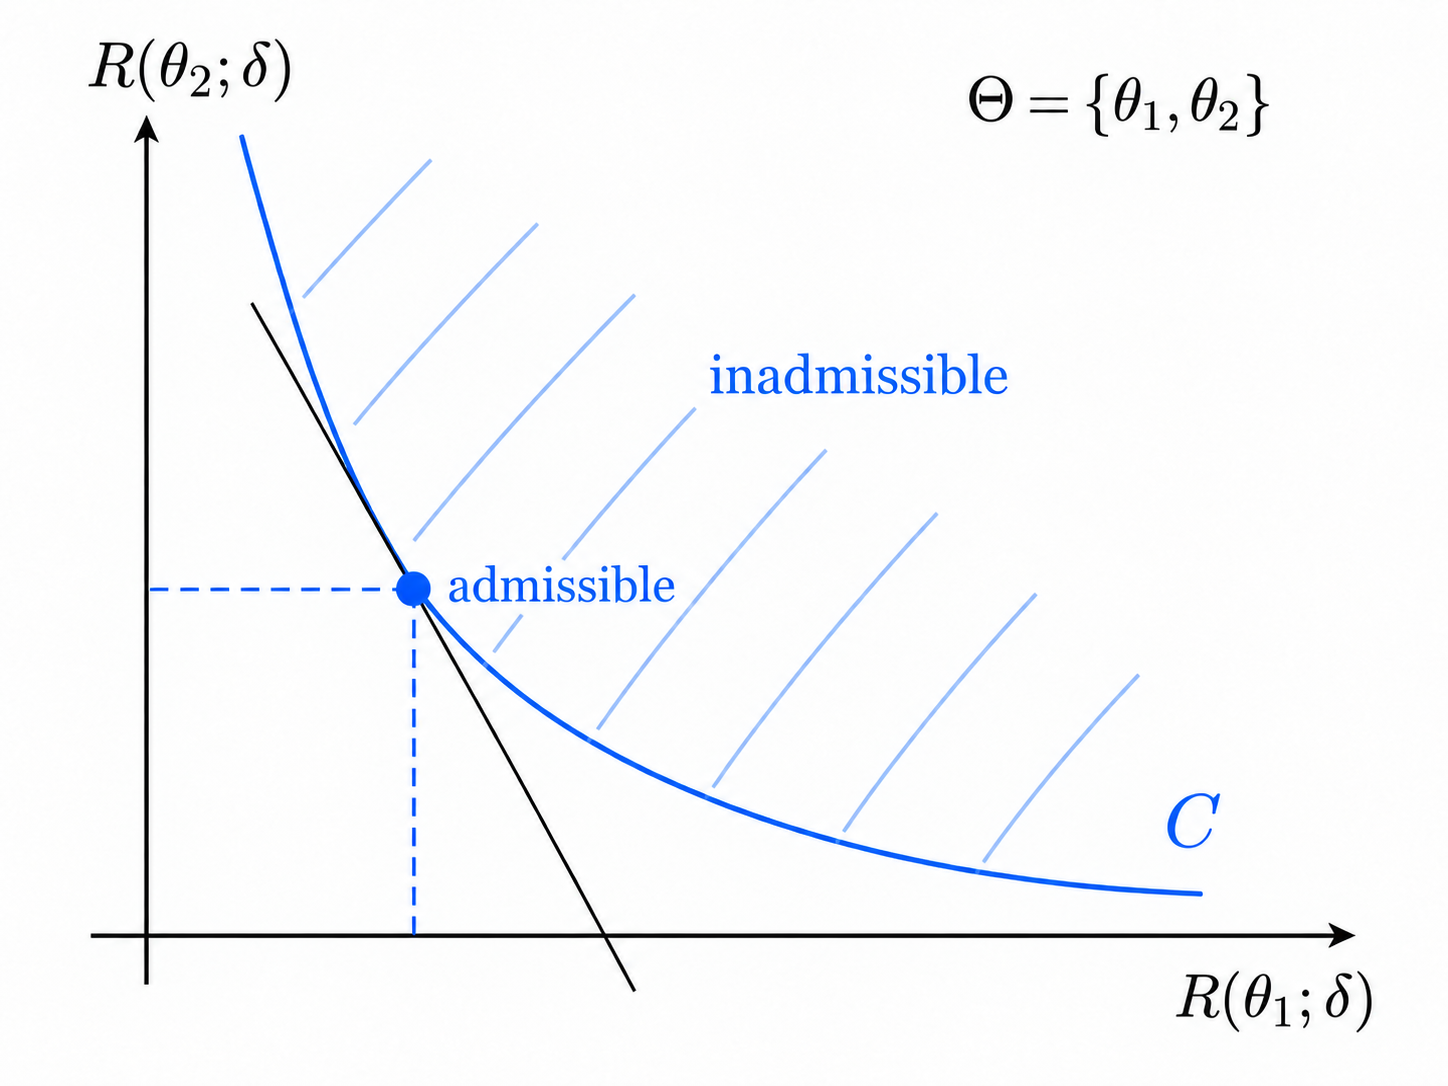
\includegraphics[width=0.62\textwidth]{./lec2-separating-hyperplane-illustration.png}

  \small Risk-set geometry when $\Theta = \{\theta_1, \theta_2\}$: an admissible risk vector lies on the lower boundary of $\mathcal{C}$ and admits a supporting hyperplane.
\end{center}
We use the following theorem in convex geometry:
\begin{theorem}[Separating hyperplane theorem]
  Let $C_1, C_2 \subseteq \real^d$ be two disjoint convex sets. Then there exists a hyperplane that separates them, i.e., there exists $w \neq 0$ and $b \in \real$ such that
  \begin{align*}
    w^\top z_1 + b \leq 0, \quad \forall z_1 \in C_1,\\
    w^\top z_2 + b \geq 0, \quad \forall z_2 \in C_2.
  \end{align*}
\end{theorem}
Using this theorem, we can find a vector $w \in \real^{|\Theta|}$ such that
\begin{align*}
  w^\top z \leq w^\top z', \quad \forall z' \in \mathcal{C},
\end{align*}
and that
\begin{align*}
  w^\top z \geq w^\top z', \quad \forall z' \in \{ z' \in \real^{|\Theta|} : z' \preceq z \}.
\end{align*}
The second condition implies that $w \succeq 0$. We can then choose the prior $\pi = w / \sum_j w_j$. Then, we have
\begin{align*}
  r_\pi (\delta) = \sum_j \pi_j R(\theta_j; \delta) = \frac{w^\top z}{\sum_j w_j} \leq \frac{w^\top z'}{\sum_j w_j} = r_\pi (\delta'), \quad \forall z' \in \mathcal{C}.
\end{align*}
This shows that $\delta$ is a Bayes rule with respect to prior $\pi$.

\section{Sufficient statistics}
Motivation: e.g., for $X_1, X_2, \cdots, X_n \simiid \mathrm{Ber} (p)$, we get some zeros and ones, and it does not matter what order they are in. Only the counts matter.

Mathematically, we note that for
\begin{align*}
  T (X_1, X_2, \cdots, X_n) = \sum_{i=1}^n X_i,
\end{align*}
the data $(X_i)_{i=1}^n$ can be reconstructed from $T$ by uniformly sampling from the set of all sequences with the same sum. This reconstruction procedure is independent of the parameter $p$.
In other words, we can safely compress the $n$ bits of information into $\log n$ bits without losing any information about the parameter $p$.

\begin{definition}
  Let $X \sim \Prob_\theta$ for $\theta \in \Theta$. A statistic $T(X)$ is called a sufficient statistic for $\theta$ if the conditional distribution of $X$ given $T(X)$ does not depend on $\theta$, i.e.,
  \begin{align*}
    \Prob_\theta (X \in A \mid T(X) = t) = \Prob_{\theta'} (X \in A \mid T(X) = t), \quad \forall A, t, \theta, \theta'.
  \end{align*}
\end{definition}
Why is this useful?
\begin{theorem}
  Let $T(X)$ be a sufficient statistic for $\theta$. Then, for any decision rule $\delta$, there exists another decision rule $\delta'$ that depends only on $T(X)$ such that
  \begin{align*}
    \delta (X) \stackrel{d}{=} \delta' (T(X)), \quad \forall \theta \in \Theta.
  \end{align*}
\end{theorem}
Operationally, this means that we can mimic the behavior of any decision rule by only looking at the sufficient statistic.

Proof: Since the conditional distribution $X \mid T (X)$ is independent of $\theta$, we can choose arbitrary $\theta_0 \in \Theta$ and sample $X' \sim \Prob_{\theta_0} (X \mid T(X))$. Then, we can define
\begin{align*}
  \delta' (T(X)) \mydefn \delta (X').
\end{align*}
\begin{theorem}[Rao--Blackwellization]
  Suppose that $T(X)$ is a sufficient statistic for $\theta$, and the loss function $L(\theta, a)$ is convex in $a$. Then, for any decision rule $\delta$, by letting
  \begin{align*}
    \eta (T (X)) \mydefn \Exs_{\theta_0} [\delta (X) \mid T(X)], \quad \mbox{for some arbitrary } \theta_0 \in \Theta,
  \end{align*}
  we have
  \begin{align*}
    R(\theta; \eta) \leq R(\theta; \delta), \quad \forall \theta \in \Theta.
  \end{align*}
\end{theorem}
Proof: straightforward application of Jensen's inequality.

Operationally, this is useful: start from some simple estimator, and then apply Rao--Blackwell\-ization to get a better estimator that depends only on the sufficient statistic. In some regime, it is known to be optimal in some sense.

\subsection{How to find sufficient statistics?}
We can verify the definition, but it involves checking conditional distributions, which is not always easy.
\begin{theorem}[factorization theorem]
  Let $X \sim \Prob_\theta$ for $\theta \in \Theta$, assuming that $\Prob_\theta$ has a density $p_\theta(x)$ with respect to some reference measure $\lambda$. Then the following are equivalent:
  \begin{enumerate}
    \item $T(X)$ is a sufficient statistic for $\theta$.
    \item There exist functions $g_\theta$ and $h$ such that
    \begin{align*}
      p_\theta (x) = g_\theta (T(x)) h(x), \quad \forall x \in \mathcal{X}, \theta \in \Theta.
    \end{align*}
  \end{enumerate}
\end{theorem}
Proof: (assuming existence of joint density)

\paragraph{$1 \Leftarrow 2$:} By Bayes' rule, we have
\begin{align*}
  p_\theta (x \mid T(X) = t) = \frac{ g_\theta (t) h (x) \bm{1}_{T(x) = t}}{\int_{ T(x') = t} g_\theta (t) h (x') d\lambda(x')} = \frac{h (x) \bm{1}_{T(x) = t}}{\int_{ T(x') = t} h (x') d\lambda(x')}.
\end{align*}
The right-hand side does not depend on $\theta$. So $T(X)$ is sufficient.
\paragraph{$1 \Rightarrow 2$:} We construct directly:
\begin{align*}
  g_\theta (t) &\mydefn \int_{T(x) = t} p_\theta (x) d\lambda(x) = p_\theta (T(X) = t),\\
  h(x) &\mydefn \frac{p_{\theta_0} (x)}{g_{\theta_0} (T(x))} = p_{\theta_0} (X = x \mid T(X) = t), \quad \text{for some arbitrary } \theta_0 \in \Theta.
\end{align*}
By sufficiency, $h (x)$ does not depend on the choice of $\theta_0$.

[If you want a more rigorous measure-theoretic proof, see Keener's textbook]

\subsection{Exponential family}
A particular family of densities that factorizes in a nice form:
\begin{align*}
  p_\theta (x) = \exp \big( \eta (\theta)^\top T (x) - B (\theta) \big) \cdot h (x),
\end{align*}
where $\eta (\theta), T(x) \in \real^k$.

By factorization, $T (X)$ is a sufficient statistic for $\theta$. Here $\eta (\theta)$ is called the natural parametrization for this exponential family.

\bigskip
\noindent \textbf{Examples}:
\begin{itemize}
  \item Multivariate Gaussian $X \sim \mathcal{N} (\mu, \Sigma)$ with unknown $\mu$ and $\Sigma$. We can factorize the density as
  \begin{align*}
    p_{\mu, \Sigma} (x) &= \frac{1}{(2\pi)^{d/2} \det(\Sigma)^{1/2}} \exp \Big( -\frac{1}{2} (x - \mu)^\top \Sigma^{-1} (x - \mu) \Big)\\
    &= \exp \Big( \underbrace{-\frac{1}{2} x^\top \Sigma^{-1} x + x^\top \Sigma^{-1} \mu}_{\eta(\mu, \Sigma)^\top T(x)} - \underbrace{\frac{1}{2} \mu^\top \Sigma^{-1} \mu - \frac{1}{2} \log\det(\Sigma) - d/2\log(2\pi)}_{B(\mu, \Sigma)} \Big).
  \end{align*}
  So we can take $T(x) = (x, xx^\top)$ as the sufficient statistic for $(\mu, \Sigma)$.
  \item $X \sim \mathcal{N} (\mu, I_d)$ with unknown $\mu$. It is also an exponential family, and $T(X) = X$ is sufficient for $\mu$.
  \item $X \sim \mathcal{N} (0, \Sigma)$ with unknown $\Sigma$. It is also an exponential family, and $T(X) = XX^\top$ is sufficient for $\Sigma$.
  \item Binomial distribution $X \sim \mathrm{Binom} (n, \theta)$ with unknown $\theta$. We have
  \begin{align*}
    p_\theta (x) = \binom{n}{x} \theta^x (1 - \theta)^{n - x} = \exp \Big(\underbrace{ x \log \frac{\theta}{1 - \theta}}_{T (x)^\top \eta (\theta)} + \underbrace{n \log (1 - \theta) }_{- B (\theta)}\Big) \cdot \underbrace{\binom{n}{x}}_{h (x)}.
  \end{align*}
  So binomial distribution is an exponential family, and $T(X) = X$ is sufficient for $\theta$.
\end{itemize}
\begin{proposition}
  Let $X_1, X_2, \cdots, X_n \simiid p_\theta$ with $p_\theta$ being from an exponential family, $p_\theta (x) = \exp \big( \eta (\theta)^\top T (x) - B (\theta) \big) \cdot h (x)$. Then we have
  \begin{align*}
    p_\theta (x_1, \cdots, x_n) = \exp \Big( \eta (\theta)^\top \sum_{i=1}^n T (x_i) - n B (\theta) \Big) \cdot \prod_{i=1}^n h (x_i)
  \end{align*}
  is also an exponential family, with sufficient statistic $T(X_1, \cdots, X_n) = \sum_{i=1}^n T (X_i)$.
\end{proposition}
Implication to multivariate normal: sample first/second moments and their combination are sufficient statistics for the mean/covariance and their combination.

\paragraph{Non-example:}\hfill\break
Uniform distribution $X \sim \mathrm{Unif} ([\theta - 1, \theta + 1])$ with unknown $\theta$. Let $X_1, X_2, \cdots, X_n \simiid \mathrm{Unif} ([\theta - 1, \theta + 1])$. Then, the joint density is
\begin{align*}
 p_\theta (x_1, \cdots, x_n) = 2^{-n} \bm{1}_{x_{(1)} \geq \theta - 1, x_{(n)} \leq \theta + 1},
\end{align*}
where $X_{(i)}$ denotes the $i$-th smallest element in the sample. This does not factorize in the exponential family form. However, we can still find a sufficient statistic $T(X_1, \cdots, X_n) = (X_{(1)}, X_{(n)})$.

\subsection{Connection between sufficiency and unbiased estimation}
Goal: estimate $g (\theta)$ from $X \sim \Prob_\theta$.
\begin{definition}
  $\delta$ is unbiased for $g (\theta)$ if
  \begin{align*}
    \Exs_\theta \big[ \delta (X) \big] = g (\theta), \quad \forall \theta \in \Theta.
  \end{align*}
\end{definition}
In general, there's no unified way of comparing estimators. That's why we have Bayes and minimax criteria. But if we restrict to unbiased estimators, we can compare them by variance.
\begin{definition}[Uniformly minimum variance unbiased estimator (UMVUE)]
  Let $\delta$ be an unbiased estimator for $g (\theta)$. We say $\delta$ is a UMVUE if for any other unbiased estimator $\delta'$ for $g (\theta)$, we have
  \begin{align*}
    \var_\theta \big[ \delta (X) \big] \leq \var_\theta \big[ \delta' (X) \big], \quad \forall \theta \in \Theta.
  \end{align*}
  UMVUE may not always exist. But there're some interesting classes of distributions where UMVUE exists and can be characterized, and it is related to sufficient statistics.

\end{definition}

\end{document}
